%%!TeX TS-program = xelatex
%!TeX encoding = UTF-8
% !TeX spellcheck = russian-aot
\documentclass[12pt, a4paper]{article}

% Basic packages
\usepackage[T1,T2A]{fontenc}
\usepackage[utf8]{inputenc}
\usepackage[english,russian]{babel}	% Localization
%\usepackage{extsizes} % Big font
%\usepackage{erewhon}  % Different font
%\setmainfont{Georgia}

% Basic packages XeLaTex
%\usepackage{xecyr}
%\usepackage[english,russian]{babel} 
%\usepackage{fontspec} 
%\defaultfontfeatures{Ligatures={TeX},Renderer=Basic}
%\setmainfont[Ligatures={TeX,Historic}]{Times New Roman} 
%\setsansfont{Comic Sans MS}
%\setmonofont{Courier New}

% Math
\usepackage{amsmath,euscript,mathrsfs}
\usepackage{amssymb,amsfonts,latexsym,mathtools}

\usepackage{caption,tabularx}

% Graphics
\usepackage{graphicx,setspace,subcaption}
\usepackage[usenames,dvipsnames,svgnames]{xcolor}

% Formatting
\usepackage[top=20mm,bottom=20mm,left=30mm,right=10mm]{geometry}
\setlength{\parindent}{1.25cm}
%\onehalfspacing
\linespread{1.15}
\usepackage{enumitem}

% Hyperlinks
\usepackage[unicode]{hyperref}
\hypersetup{
	colorlinks=true,
	linkcolor={black!50!black},
	citecolor={blue!50!black},
	urlcolor={blue!50!black},
}

%\mathtoolsset{showonlyrefs=true}

% Dots in section titles
%\renewcommand{\thechapter}{\arabic{chapter}.}
%\renewcommand{\thesection}{\thechapter.\arabic{section}.}
%\renewcommand{\thesubsection}{\thesection.\arabic{subsection}.}

% Rename some sections
%\addto\captionsrussian{\def\contentsname{Содержание}}
%\addto\captionsrussian{\def\bibname{Список источников}}

%\renewcommand\contentsname{Содержание}
%\renewcommand\refname{Список источников}
%\renewcommand{\printtoctitle}[1]{\Huge\sffamily #1}

% Smaller chapter title
%\usepackage{titlesec}
%\titleformat{\chapter}[display]
%{\bfseries\Large}%
%{\chaptertitlename\hspace{1ex}\thechapter.}%
%{2 pt}%
%{\bfseries\Large}%
%%\titleformat*{\section}{\thesection \Large}
%%\titleformat{\section}{}{}{\normalfont\bfseries}{\thesection}
%\titleformat{\section}{\bfseries\large}{\thesection.}{.5em}{}
%\titleformat{\subsection}{\bfseries}{\thesubsection.}{.5em}{}
%
%\titlespacing*{\chapter}{0pt}{0pt}{40pt}

% Dots in table of contents
%\usepackage{tocloft}
%\renewcommand{\cftchapleader}{\cftdotfill{\cftdotsep}} % for chapters

% Graphics path for figures
\graphicspath{{figures/}}

% Absolute value declaration
\DeclarePairedDelimiter{\abs}{\lvert}{\rvert}
\DeclarePairedDelimiter{\norm}{\|}{\|}
\DeclareMathOperator{\erf}{erf}
\DeclareMathOperator{\trace}{tr}
%\DeclareMathOperator{\tg}{tg}
%\DeclareMathOperator{\ctg}{ctg}
\DeclareMathOperator{\sech}{sech}

% Page breaking in multi-line formulae
\allowdisplaybreaks[1]

% Delimiters
\newcommand{\lb}{\left (}
\newcommand{\rb}{\right )}
\newcommand{\lset}{\left \{}
\newcommand{\rset}{\right \}}
\newcommand{\lsq}{\left [}
\newcommand{\rsq}{\right ]}

% Tensors
\newcommand{\vect}[1]{\underline{#1}}
\newcommand{\tens}[1]{\underline{\underline{#1}}}

% Additional commands
\newcommand{\divg}{\text{div}}

% Big 'O' notation
\renewcommand{\O}[1]{O \lb #1 \rb}

% Equation specific commands
\newcommand{\eqtext}[1]{\quad \text{#1} \quad}
\newcommand{\RA}{\quad \Rightarrow \quad}

% Derivatives (normal and partial)
\newcommand{\dd}[1]{\; \mathrm{d} #1}
\newcommand{\diff}[2]{\frac{\mathrm{d} #1}{\mathrm{d} #2}}
\newcommand{\diffn}[3]{\dfrac{\mathrm{d}^{#1} #2}{\mathrm{d} #3^{#1}}}
\newcommand{\pdd}[1]{\; \partial #1}
\newcommand{\pdiff}[2]{\frac{\partial #1}{\partial #2}}
\newcommand{\pdiffn}[3]{\dfrac{\partial^{#1} #2}{\partial #3^{#1}}}


\begin{document}

\begin{titlepage}
	\newgeometry{top=20mm,bottom=15mm,left=25mm,right=15mm}
	
	\begin{center}
		\vspace*{80mm}
		{РЕФЕРАТ ПО ТЕМЕ МАГИСТЕРСКОЙ ДИССЕРТАЦИИ}\\
		\vspace{5mm} 
		{\bf ПРОДОЛЬНЫЕ ВОЛНЫ ДЕФОРМАЦИИ В НЕЛИНЕЙНО УПРУГИХ ВОЛНОВОДАХ}
	\end{center}

	\vspace{30mm}
	\begin{flushleft}
	\begin{tabularx}{\linewidth}{Xr}
		Выполнил & Ф.\,E.~Гарбузов  \\ 
		\vspace{3mm}
		Руководитель &  \\ 
		проф., д.т.н. & Б.\,С.~Григорьев \\ 
		\vspace{3mm}
		Научный консультант  &  \\ 
		к.ф.-м.н. & Я.\,М.~Бельтюков
	\end{tabularx} 
	\end{flushleft}

	
	\vspace{50mm}
	
	\begin{center}
		Санкт-Петербург\\2019
	\end{center}
	
\end{titlepage}



\section{Введение}
\setcounter{page}{2}

Исследование волн деформации в нелинейно упругих телах
является важной темой современного изучения волн.
Начиная с 1970\babelhyphen{nobreak}х годов опубликован ряд работ, в которых выводились упрощённые асимптотические модели типа Буссинеска и Кортевега--де Фриза для описания длинных продольных волн малой амплитуды в волноводах разной геометрии~\cite{OS, NS, S_book, P_book, SP, DC, DF, KSZ}. Эти модели имеют семейства точных решений в виде уединённых волн --- солитонов деформации.

В литературе обсуждается гипотетическая возможность применения солитонов деформации в задачах дефектоскопии, поскольку, как показано в недавних работах \cite{KS, KT1, KT2}, солитоны сохраняют память о прохождении через область с дефектом (например, с расслоением). В ФТИ им. Иоффе много лет ведётся работа по экспериментальному обнаружению солитонов деформации \cite{JAP2010, JAP2012}, однако до сих пор надёжных данных об их существовании нет. Ввиду этого представляет интерес построение моделей, учитывающих внешнее воздействие на волновод, с целью моделирования возникновения солитонов в результате воздействия внешних сил. 

В настоящей работе мы рассмотрели нелинейные волны в однородных стержнях круглого сечения. Во-первых, следуя асимптотическому подходу, схожему с использовавшимся в ранее опубликованных работах, мы получили новую модель типа Буссинеска, учитывающую осесимметричную нагрузку на боковой поверхности стержня. Во-вторых, на основе многодоменного псевдоспектрального метода нам удалось построить эффективный численный метод для решения полных уравнений, описывающих динамику нелинейно упругого стержня. Мы провели численное моделирование ряда начально-краевых задач, в ходе которых возникали солитоны, и сравнили параметры солитонов в полной модели и упрощённой модели типа Буссинеска.

\section{Нелинейная теория упругости}
В рамках линейной теории упругости потенциальная энергия деформации включает в себя только слагаемые второго порядка относительно градиента вектора перемещения, в то время как в нелинейной теории учитываются слагаемые более высоких порядков. В случае слабой нелинейности (малых, но конечных деформаций) общей моделью для потенциальной энергии является модель Мурнагана:
\begin{equation}\label{murnaghan}
W = \frac{\lambda + 2\mu}{2}I_1(\tens{E})^2 - 2\mu I_2(\tens{E}) + \frac{l+2m}{3}I_1(\tens{E})^3 - 2m I_1(\tens{E}) I_2(\tens{E}) + n I_3(\tens{E}),
\end{equation}
где $I_1(\tens{E}) = \trace \tens{E},\  I_2(\tens{E}) = \lsq(\trace \tens{E})^2 - \trace \tens{E}^2\rsq/\,2,\ I_3(\tens{E}) = \det \tens{E}$ --- инварианты тензора; $\lambda$ и $\mu$ --- коэффициенты упругости Ламе; $l$, $m$, $n$ --- упругие модули Мурнагана; а тензор конечных деформаций Грина записывается следующим образом ($\vect{U}$ --- вектор перемещения):
\begin{equation}\label{1_strain}
\tens{E} = \frac12 \lb(\nabla\vect{U})^T + \nabla\vect{U} + (\nabla\vect{U})^T\cdot\nabla\vect{U}\rb.
\end{equation}
Полные уравнения движения стержня в отсутствие массовых сил записываются в векторном виде следующим образом:
\begin{equation}\label{full_eqns}
\rho\ddot{\vect{U}} = \divg\tens{P}, \qquad \tens{P} = (\tens{I} + \nabla\vect{U}) \cdot \pdiff{W}{\tens{E}},
\end{equation}
где $P$ --- первый тензор напряжений Пиолы-Кирхгофа, а $\tens{I}$ --- единичный тензор.


\section{Вывод упрощённой системы двух связанных уравнений}

Рассмотрим стержень круглого поперечного сечения радиуса $R$. Введём цилиндрическую систему координат $(x, r, \varphi)$, где $x$ -- осевая координата, $r$ -- продольная, $\varphi$ -- угловая, как показано на рисунке \ref{fig:rod}. Положим стержень бесконечным вдоль оси $x$. Используя Лагранжев подход, введём вектор перемещения точек тела: $\vect{U} = (U, V, W)$, где $U$ -- осевое (продольное) перемещение, $V$ -- радиальное (поперечное) перемещение, а $W$ -- вращение.
\begin{figure}[h]
	\centering
	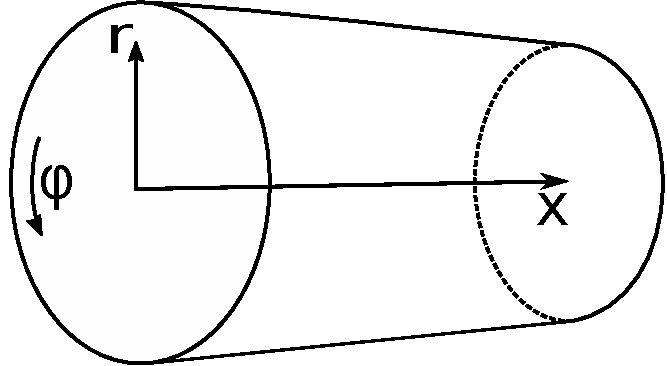
\includegraphics[width=0.3\textwidth]{1_RodSchematic}
	\caption{Стержень с круглым поперечным сечением.}
	\label{fig:rod}
\end{figure}

Рассмотрим задачу, в которой отсутствует кручение стержня, а продольное и поперечное перемещения не зависят от угла $\varphi$:
\begin{equation}\label{2_assumptions}
U = U(x,r,t), \quad V = V(x,r,t), \quad W = 0.
\end{equation}
Уравнения движения, в условиях \eqref{2_assumptions} и отсутствия массовых сил, принимают вид
\begin{align}
\label{2_eq1_0}
&\rho  \frac{\partial^2 U(x,r,t)}{\partial t^2}-\frac{\partial P_{x x}}{\partial x}-\frac{\partial P_{xr}}{\partial r}-\frac{P_{xr}}{r} = 0,\\
\label{2_eq2_0}
&\rho  \frac{\partial^2 V(x,r,t)}{\partial t^2} - \frac{\partial P_{rx}}{\partial x}-\frac{\partial P_{rr}}{\partial r}-\frac{P_{rr} - P_{\varphi\varphi}}{r} = 0,
\end{align}
а третье уравнение представляется в виде тождества $0\equiv 0$. Здесь $P_{\alpha \beta}$ обозначает компоненту первого тензора Пиолы-Кирхгофа. Задавая на поверхности стержня осесимметричное напряжение $\vect{P_b} = (P(x,t), T(x,t), 0)$, получаем граничные условия в виде:
\begin{align}
P_{rr} &= P(x, t) \quad \mbox{при} \quad r = R \label{2_bc_rr},\\
P_{xr} &= T(x, t) \quad \mbox{при} \quad r = R \label{2_bc_rx}.
\end{align}
Поскольку компонента $ P_{\varphi r} \equiv 0 $, третье граничное условие $P_{\varphi r} = 0$ при $r = R$ выполняется автоматически.

Следуя обсуждавшимся во введении работам и аналогичным исследованиям в рамках линейной упругости \cite{bostrm2000}, будем искать решение в виде степенного ряда по радиальной координате:
\begin{align}
\label{u_series}
U(x,r,t) &= U_0(x,t) + r^2 U_2(x,t) + r^4 U_4(x,t) + \dots \, ,\\
\label{v_series}
V(x,r,t) &= r V_1(x,t) + r^3 V_3(x,t) + r^5 V_5(x,t) + \dots \, .
\end{align}

Введём масштабные множители, выделяющие среди прочих задачу о распространении длинных по сравнению с радиусом стержня волн малой амплитуды. Тогда безразмерные переменные и функции определяются следующими выражениями:
\begin{equation} \label{scales1}
\tilde t = \frac{t}{L/c}, \quad \tilde x = \frac{x}{L}, \quad \tilde r = \frac{r}{L}, \quad \tilde U = \frac{U}{\varepsilon L}, \quad \tilde V = \frac{V}{\varepsilon L}, \quad \tilde P = \frac{P}{E \varepsilon}, \quad \tilde T = \frac{T}{E \varepsilon\delta},
\end{equation}
из которых следует, что
$\tilde U_n = L^{n-1} U_n/\varepsilon, \ \tilde V_n =  L^{n-1} V_n/\varepsilon$ для $n \geqslant 0$.
Здесь $L$ является характерной длиной волны, $c$ -- скорость линейной волны, $E$ -- модуль Юнга, $\varepsilon \ll 1$ --- малый параметр амплитуды, $\displaystyle \delta = R/L \ll 1$ --- второй малый параметр, а тильда обозначает безразмерную величину. Отметим, что при таком выборе масштабов переменная $\tilde r$ принимает значения от $0$ до $\delta$ и является малой величиной.
В дальнейшем мы опустим тильду над безразмерными величинами.

Подстановка \eqref{u_series}, \eqref{v_series} в уравнения движения \eqref{2_eq1_0}, \eqref{2_eq2_0} и приравнивание к нулю коэффициентов при различных степенях $r$ позволяет выразить все старшие члены разложений ($U_2$, $V_3$, $U_4$) через первые ($U_0$ и $V_1$), представляя их в виде ряда по малому параметру $\varepsilon$:
\begin{align}
\label{U2}
U_2 &= \frac{1}{4\mu} \left[ \rho c^2 U_{0tt} - (\lambda + 2\mu) U_{0xx} - 2(\lambda + \mu) V_{1x} \right] + \varepsilon f_2(x,t) + O(\varepsilon^2),\\
\label{V3}
V_3 &= \frac{1}{8(\lambda + 2\mu)} \left[ \rho c^2 V_{1tt} - 2(\lambda + \mu) U_{2x} - \mu V_{1xx} \right] + \varepsilon f_3(x,t) + O(\varepsilon^2),\\
\label{U4}
U_4 &= \frac{1}{16\mu}\left[\rho c^2 U_{2tt} - (\lambda + 2\mu) U_{2xx} - 4(\lambda + \mu) V_{3x}\right] + O(\varepsilon).
%V_5 &=& \frac{1}{24(\lambda + 2\mu)} \left(\rho c^2 V_{3tt} - 4(\lambda+\mu)U_{4x} - \mu V_{3xx}\right) + O(\varepsilon).
\end{align}
Здесь $x$ и $t$ в нижнем индексе обозначает частную производную по соответствующей переменной, а выражения для нелинейных функций $f_2$ и $f_3$ очень громоздки и не приводятся здесь.

Подстановка функций $ U_2 $, $ V_3 $, $ U_4 $ в граничные условия \eqref{2_bc_rr}, \eqref{2_bc_rx} приводит к следующей системе уравнений:
\begin{equation} \label{2_bc_rr_subst}
\begin{split}
2 (\lambda + \mu) V_1 + \lambda U_{0x} &+\varepsilon \Psi_1(U_0, V_1) + \frac{\delta^2}{8} \bigg[ (\lambda + 3\mu) U_{0xxx}- \frac{\rho c^2(\lambda + 3\mu)}{\lambda + 2\mu} U_{0xtt} \\
&+ \frac{2\rho c^2(2\lambda + 3\mu)}{\lambda + 2\mu} V_{1tt} + 2\lambda V_{1xx}\bigg] 
+ O(\varepsilon^2, \varepsilon\delta^2, \delta^4) =  \frac{\mu(3\lambda + 2\mu)}{\lambda + \mu} P,
\end{split}
\end{equation}
\begin{equation} \label{2_bc_rx_subst}
\begin{split}
\rho  c^2 U_{0tt} -2 \lambda  V_{1x}-(\lambda +2 \mu ) U_{0xx} - \varepsilon \Psi_2(U_0, V_1)
+ \frac{\delta^2}{8}\bigg[(3\lambda + 4\mu)U_{0xxxx} + \frac{\rho^2 c^4}{\mu}U_{0tttt}\\
- \frac{\rho c^2\left(\lambda^2 + 7\lambda\mu + 8\mu^2\right)}{\mu(\lambda + 2\mu)} U_{0xxtt} + 2(3\lambda + 2\mu)V_{1xxx} - \frac{2 \rho  c^2 \left(\lambda ^2+4 \lambda  \mu +2 \mu ^2\right)}{\mu(\lambda + 2\mu)} V_{1xtt} \bigg]\\
+\,O(\varepsilon^2, \varepsilon\delta^2, \delta^4)
= \frac{2\mu(3\lambda + 2\mu)}{\lambda + \mu} T,
\end{split}
\end{equation}
где нелинейные члены выражаются следующим образом: 
\begin{align}
	\nonumber
	\Psi_1 &= (4l + 2m + 3\lambda + 3\mu) V_1^2 + (4l - 2m + n + \lambda) U_{0x} V_1 + \frac{1}{2} (2l + \lambda) U_{0x}^2, \\
	\nonumber
	\Psi_2 &= \left((4l - 2m + n + \lambda) V_1^2 + 2(2l + \lambda) U_{0x} V_1 + \frac12(2l + 4m + 3\lambda + 6\mu) U_{0x}^2 \right)_x.
\end{align}
Эта система связанных уравнений представляет собой довольно сложную модель, однако она может быть сведена к одному уравнению типа Буссинеска.


\section{Вывод уравнения типа Буссинеска}
Существует два естественных способа вывода модели типа Буссинеска. В первом способе исключение функции $V_1$ из уравнений \eqref{2_bc_rr_subst} и \eqref{2_bc_rx_subst} осуществляется с помощью асимптотического выражения, следующего из уравнения \eqref{2_bc_rr_subst}:
\begin{equation} \label{v1_asympt}
V_1(x, t) = \frac{\mu(3\lambda + 2\mu) P}{2(\lambda + \mu)^2} - \frac{\lambda U_{0x}}{2(\lambda + \mu)} + \varepsilon f(x,t) + \delta^2 g(x,t) + O(\varepsilon^2, \varepsilon\delta^2, \delta^4),
\end{equation}
где неизвестные функции $f$ и $g$ ищутся из условия равенства нулю коэффициентов при $\varepsilon$ и $\delta^2$ в \eqref{2_bc_rr_subst}. Затем, подстановка $V_1$ в \eqref{2_bc_rx_subst} приводит к следующему уравнению типа Буссинеска относительно $U_0$:
\begin{equation} \label{eq_u0_asympt}
\begin{split}
&\rho c^2 U_{0tt} - \frac{\mu(3\lambda + 2\mu)}{\lambda + \mu}\left(U_{0xx} + \frac{\lambda}{\lambda + \mu} P_x + 2T\right) - \varepsilon \left(\gamma_1 U_{0x}^2 + \gamma_2 U_x P + \gamma_3 P^2 \right)_x \\
&\quad+ \delta^2 \bigg[\frac{\rho ^2 c^4 U_{0tttt}}{8\mu} + \frac{\mu (3\lambda + 2\mu)^2 U_{0xxxx}}{8(\lambda + \mu)^2} - \frac{\rho c^2 \left(7\lambda^2 + 10\lambda\mu + 4\mu^2\right) U_{0xxtt}}{8(\lambda + \mu)^2} + F(P, T) \bigg]\\
&\hspace{117mm}+ O(\varepsilon^2, \varepsilon\delta^2, \delta^4) = 0.
\end{split}
\end{equation}
Коэффициенты $\gamma_1$, $\gamma_2$, $\gamma_3$ и функция $F$ громоздки и не приводятся здесь.

Другой метод основан на точном, а не асимптотическом исключении $V_1$ из линейной части уравнений \eqref{2_bc_rr_subst} и \eqref{2_bc_rx_subst}.
Уравнения \eqref{2_bc_rr_subst} и \eqref{2_bc_rx_subst} могут быть записаны в следующем виде:
\begin{align}%\label{key}
L_{1} V_1 + \varepsilon\Psi_1(U_0, V_1) &= a_1 P + M_1 U_0 + O(\varepsilon^2, \varepsilon\delta^2, \delta^4),\\
L_{2} V_1 + \varepsilon\Psi_2(U_0, V_1) &= a_2 T + M_2 U_0 + O(\varepsilon^2, \varepsilon\delta^2, \delta^4),
\end{align}
где $a_1$ и $a_2$ --- константы; $L_{1}$, $L_{2}$, $M_{1}$ и $M_{2}$ -- линейные дифференциальные операторы, действующие на $V_1$ и $U_0$ соответственно в уравнениях \eqref{2_bc_rr_subst} и \eqref{2_bc_rx_subst}. Теперь, применяя $L_{2}$ к первому уравнению, $L_{1}$ ко второму и вычитая одно уравнение из другого, получаем:
\begin{equation}
\varepsilon [L_{2}\Psi_1(U_0, V_1) - L_{1}\Psi_2(U_0, V_1)] =  L_{2}\lb a_1 P + M_1 U_0\rb - L_{1}\lb a_2 T + M_2 U_0\rb + O(\varepsilon^2, \varepsilon\delta^2, \delta^4).
\end{equation}
Чтобы исключить $V_1$ из нелинейной части приходится воспользоваться асимптотическим выражением \eqref{v1_asympt}, что приводит к следующему уравнению:
\begin{equation} \label{eq_u0_bostr}
\begin{split}
%\nonumber
\rho c^2 U_{0tt} &- \frac{\mu(3\lambda + 2\mu)}{\lambda + \mu} \left(U_{0xx} + \frac{\lambda}{\lambda + \mu} P_x + 2T\right)
- \varepsilon \left(\gamma_1 U_{0x}^2 + \gamma_2 U_x P + \gamma_3 P^2 \right)_x \\
&\hspace{15mm}+ \delta^2 \bigg[\frac{\rho ^2 c^4 (\lambda^2 + 5\lambda\mu + 5\mu^2) U_{0tttt}}{8\mu(\lambda+2\mu)(\lambda+\mu)} - \frac{\rho c^2 \left(6\lambda^2 + 21\lambda \mu + 14\mu^2\right) U_{0xxtt}}{8(\lambda + 2\mu)(\lambda + \mu)} \\
&\hspace{45mm} + \frac{\mu(3\lambda + 2\mu) U_{0xxxx}}{4(\lambda + \mu)} + G(P, T)\bigg] + O(\varepsilon^2, \varepsilon\delta^2, \delta^4) = 0.
\end{split} 
\end{equation}
%Отметим, что в линейном приближении при $\varepsilon = 0$ уравнение \eqref{eq_u0_bostr} совпадает с уравнениями, выведенными для линейной задачи в~\cite{bostrm2000}.
%Из \eqref{eq_u0_asympt} и \eqref{eq_u0_bostr}, задавая $\varepsilon = 0$, $\delta = 0$ и $P = T = 0$, получаем скорость линейной продольной волны в бесконечно тонком стержне:
%\begin{equation}
%\label{lin_velocity}
%c = \ \sqrt{\frac{\mu(3\lambda + 2\mu)}{\rho(\lambda+\mu)}} = \sqrt{\frac{E}{\rho}}.
%\end{equation}
Теперь, предполагая, что коэффициенты при нелинейных и дисперсионных слагаемых в уравнениях \eqref{eq_u0_asympt} и \eqref{eq_u0_bostr} являются величинами одного порядка ($ \varepsilon \sim \delta^2 $), можно отбросить слагаемые $O(\varepsilon^2, \varepsilon\delta^2, \delta^4)$. 

Полученные уравнения записаны относительно перемещения $U_0$, однако основной интерес представляют значения не перемещения, а деформации. Продифференцируем уравнения \eqref{eq_u0_asympt} и \eqref{eq_u0_bostr} по $x$ и введём новую функцию $u = U_{0x}$, характеризующую продольную деформацию. Получаемые в результате уравнения мы запишем в размерном виде, вместо упругих модулей Ламе $\lambda$ и $\mu$ подставим их выражения через модуль Юнга $E$ и коэффициент Пуассона $\nu$, а также учтём, что $c=\sqrt{E/\rho}$:
\begin{equation}\label{eq_dim}
\begin{split}
&u_{tt} - c^2 u_{xx} - \frac{2}{\rho}\bigg(\nu P_{xx} + \frac1R T_x\bigg) - \left(\frac{\beta_1}{2\rho} u^2 + \frac{\beta_2}{\rho E} u P + \frac{\beta_3}{2\rho E^2} P^2\right)_{xx}\\
&\hspace{20mm} + R^2 \bigg(\frac{\alpha_1^{(i)}}{c^2} u_{tttt} + \alpha_2^{(i)} u_{xxtt} + c^2\alpha_3^{(i)} u_{xxxx} + G^{(i)}(P, T) \bigg) = 0, \quad i = 1,2,
\end{split}
\end{equation}
где $i=1$ соответствует уравнению \eqref{eq_u0_asympt}, а $i=2$ уравнению \eqref{eq_u0_bostr}, а коэффициенты принимают следующий вид:
\begin{align}
\label{beta_1}
&\beta_1 = 3E + 2l(1 - 2\nu)^3 + 4m(1 + \nu)^2 (1 - 2\nu) + 6n\nu^2,\\
\label{beta_2}
&\beta_2 = 2 (1 + \nu) \left[2 l (1 - 2 \nu)^3 + \nu \left(E + 4m \left(1 - \nu - 2\nu^2\right) - 2n (1 - 2\nu)\right) \right],\\
\label{beta_3}
&\beta_3 = 2(1 + \nu)(1 - 2 \nu) \Big[ (1 + \nu)(1 - 2\nu) [4l \left(1 - 2\nu\right) - 2m(1 + 2\nu) + n] - 2\nu E \Big]\\
\label{alpha_1}
&\alpha_1^{(1)} = \alpha_3^{(1)} = \frac{1 + \nu}{4}, \quad \alpha_2^{(1)} = -\frac{1 + \nu + \nu^2}{2}, \\
\label{alpha_2}
&\alpha_1^{(2)} = \frac{5 - 5\nu - 6\nu^2 + 4\nu^3}{8(1-\nu)},\quad \alpha_2^{(2)} = -\frac{7 - 7\nu - 2\nu^2}{8(1-\nu)}, \quad \alpha_3^{(2)} = \frac14,\\
\label{G1}
&G^{(1)} = \frac{1 + \nu + 2\nu^2}{4\rho} P_{xxxx} - \frac{1 - \nu + 2\nu^2 + 4\nu^3}{4E} P_{xxtt},\\
\label{G2}
&G^{(2)} = \frac{1 + \nu}{4\rho} P_{xxxx} - \frac{1 + \nu - 2\nu^2 - 2\nu^3}{4E(1 - \nu)} P_{xxtt} - \frac{3 - 5\nu - 4\nu^2 + 4\nu^3}{8ER(1 - \nu)} T_{xtt} - \frac{\nu}{2\rho R} T_{xxx}.
\end{align}
В случае условия свободной поверхности, т.е. $P = T = 0$, уравнения \eqref{eq_dim} сводятся к
\begin{equation}\label{eq_dim_free_surf}
u_{tt} - c^2 u_{xx} = \frac{\beta_1}{2\rho}\left(u^2\right)_{xx} -  R^2 \bigg(\frac{\alpha_1^{(i)}}{c^2} u_{tttt} + \alpha_2^{(i)} u_{xxtt} + c^2\alpha_3^{(i)} u_{xxxx}\bigg), \quad i = 1,2.
\end{equation}

Сравним оба уравнения \eqref{eq_dim_free_surf} с <<уравнением с двумя дисперсиями>>, полученным Самсоновым и Порубовым~\cite{SP}
и <<регуляризованным>> уравнением, выведенным Островским и Сутиным~\cite{OS}. Эти уравнения могут быть записаны в форме уравнений \eqref{eq_dim} с помощью следующих дисперсионных коэффициентов:
\begin{align} \nonumber
&\alpha_1^{(3)} = 0,& &\alpha_2^{(3)} = \frac{(1-\nu)\nu}{2},&  &\alpha_3^{(3)} = -\frac \nu 2,\\
\nonumber
&\alpha_1^{(4)} = 0,& &\alpha_2^{(4)} = -\frac{\nu^2}{2},&  &\alpha_3^{(4)} = 0,
\end{align}
для уравнения Самсонова--Порубова и регуляризованного уравнения соответственно.

Поясним подробнее что значит <<регуляризация>>. Все четыре приведённые выше модели не являются асимптотически точными уравнениями, т.е. в безразмерной форме они содержат как члены $ O(1) $, так и $ O(\varepsilon, \delta^2) $. Следовательно, все эти уравнения могут быть <<регуляризованы>> (сведены) к одному уравнению, в котором есть только одно дисперсионное слагаемое, используя асимптотическое соотношение $u_{tt} = c^2 u_{xx} + \mbox{<\,малые члены\,>}$. Коэффициент при этом дисперсионном слагаемом определяется суммой дисперсионных коэффициентов $\alpha_j$ и одинаков для всех четырех уравнений:
\begin{equation} \label{alpha_sum}
\alpha_1^{(i)} + \alpha_2^{(i)} + \alpha_3^{(i)} = -\frac{\nu^2}{2}, \quad i = \overline{1,4},
\end{equation}
что означает, что эти уравнения асимптотически эквивалентны.

Регуляризация может быть применена и к уравнению с внешним воздействием \eqref{eq_dim} в виде $u_{tt} = c^2 u_{xx} +  \frac{2}{\rho}\lb\nu P_{xx} + \frac1R T_x\rb + \mbox{<\,мал. члены\,>}$. Получаемое таким образом уравнение имеет вид:
%Применяя асимптотическое соотношение $u_{tt} = c^2 u_{xx} +  \frac{2}{\rho}\lb\nu P_{xx} + \frac1R T_x\rb + \mbox{<\,мал. члены\,>}$ к уравнению \eqref{eq_dim}, получаем регуляризованную модель с внешним воздействием:
%Регуляризация может быть применена и к уравнению с внешним воздействием \eqref{eq_dim}:%, что приводит к
%Поскольку модель с одним дисперсионным членом проще, чем модель с тремя дисперсионными членами, представляется целесообразным получить регуляризованную модель в случае ненулевых напряжений на поверхности:
\begin{equation}\label{2_eq_fin_reg}
\begin{split}
&u_{tt} - c^2 u_{xx} - \frac{2}{\rho}\bigg(\nu P_{xx} + \frac1R T_x\bigg) - \left(\frac{\beta_1}{2\rho} u^2 + \frac{\beta_2}{\rho E} u P + \frac{\beta_3}{2\rho E^2} P^2\right)_{xx} - \frac{\nu^2 R^2}{2} u_{xxtt}\\
& + \frac{R^2}{4} \lb\frac{1-\nu}{\rho}P_{xxxx} - \frac{1-3\nu+4\nu^3}{E}P_{xxtt}\rb + \frac{(1+\nu)R}{2}\lb \frac{1}{E}T_{xtt} - \frac{1}{\rho}T_{xxx} \rb = 0, \quad i = 1,2.
\end{split}
\end{equation}

Некоторые исследователи рассматривали задачу о распространении длинных продольных волн в предварительно растянутом стержне~\cite{DC}, поэтому для систематичности исследования мы рассмотрели и такую задачу. 
Продольное равномерное осевое растяжение задаётся в виде:
\begin{equation}\label{pre_stretch_u}
U^*(x) = \kappa x,
\end{equation}
где $\kappa$ -- постоянная, что приводит, следуя описанному выше выводу, к несколько модифицированному уравнению \eqref{eq_dim}:
\begin{equation}\label{pre_stretch_eq_dim}
\begin{split}
u_{tt} - \left(c^2 + \kappa\frac{\beta_1}{\rho}\right) u_{xx} - \frac{2}{\rho}\left[\left(\nu + \kappa \frac{\beta_2}{2E} \right) P_{xx} + \frac1R T_x\right] - \left(\frac{\beta_1}{2\rho} u^2 + \frac{\beta_2}{\rho E} u P + \frac{\beta_3}{2\rho E^2} P^2\right)_{xx}\\
+ R^2 \left(\frac{\alpha_1^{(i)}}{c^2} u_{tttt} + \alpha_2^{(i)} u_{xxtt} + c^2\alpha_3^{(i)} u_{xxxx} + G^{(i)}(P, T) \right) = 0, \quad i = 1,2.
\end{split}
\end{equation}
Предварительное растяжение изменило скорость длинных линейных волн, квадрат которой равен коэффициенту при $u_{xx}$, сделав её зависимой от коэффициента $\beta_1$, содержащего упругие модули Мурнагана. Это явление, называемое акустоэластическим эффектом, лежит в основе экспериментального определения модулей Мурнагана.

Насколько известно автору, обе модели, описываемые уравнениями (\ref{pre_stretch_eq_dim}), а также их упрощённые версии (\ref{eq_dim}), (\ref{eq_dim_free_surf}) и \eqref{2_eq_fin_reg} получены впервые. 
%В следующем параграфе мы проанализируем свойства полученных уравнений и сравним их с уравнениями выведенными ранее.



\section{Дисперсионные свойства и солитонные решения}

На рисунке \ref{fig:disp} представлены дисперсионные кривые четырёх упрощённых (с нулевыми напряжениями на поверхности и без предварительного растяжения) линеаризованных уравнения типа Буссинеска, приведённые в предыдущих разделах, а также нижние три ветви точного дисперсионного соотношения Похгаммера-Кри для линейной задачи.
\begin{figure}[h]
	\centering
	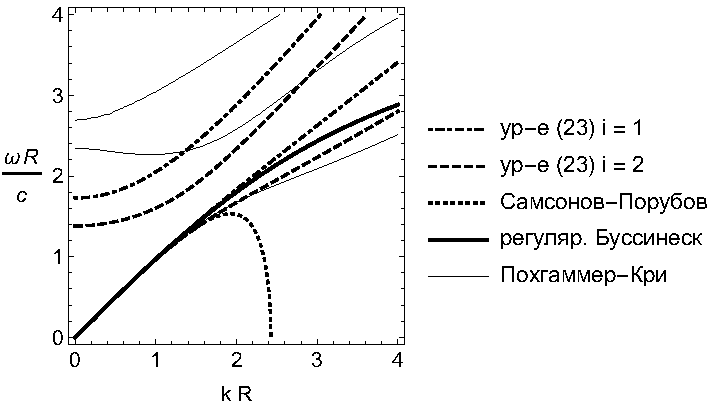
\includegraphics[width=0.65\linewidth]{2_DispBlackSmall}
	\caption{Дисперсионные кривые для стержня с $\nu = 0.34$.}
	\label{fig:disp}
	\vspace{-2mm}
\end{figure} 

Все модели достаточно хорошо описывают нижнюю ветвь дисперсионной кривой в длинноволновой области, однако наиболее точной является модель (\ref{eq_dim_free_surf}, $i=2$), что объясняется более аккуратной процедурой исключения функции $V_1$ из уравнений \eqref{2_bc_rr_subst} и \eqref{2_bc_rx_subst}. Уравнение Самсонова -- Порубова обладает коротковолновой неустойчивостью, в то время как остальные три модели не имеют такого эффекта. 
%Отметим, что коротковолновая неустойчивость затрудняет численный счёт, поскольку высокочастотные гармоники в таком случае могут неограниченно возрастать. 
Полученные в настоящей работе уравнения \eqref{eq_dim_free_surf} в отличие от других уравнений улавливают вторую ветвь дисперсионной кривой, правда описывают её очень неточно: помимо большого отличия по значению, эти кривые имеют всюду положительный наклон, тогда как точная кривая имеет отрицательный наклон в области длинных волн, что соответствует отрицательной групповой скорости.
%Уравнение (\ref{eq_dim_free_surf}, $i=2$) лучше описывает нижнюю ветвь для коротких волн, в то время как (\ref{eq_dim_free_surf}, $i=1$) обладает лучшими дисперсионными свойствами как длинноволновая модель.

%Отметим, что улавливание ещё одной моды колебаний в численном моделировании является скорее недостатком, чем преимуществом, поскольку к длинным продольным волнам, для изучения которых была построена модель, подмешиваются другие колебания.
%All models reasonably well describe the lowest branch of the dispersion curves for the long waves. Eq. (\ref{eq_dim_SP})  suffers from a short-wave instability, while other three models do not have this defect. Eq. (\ref{eq_dim_free_surf}) for $i=1,2$, capture the presence of the second branch. We also note that, at least in this example, eq. (\ref{eq_dim_free_surf}) for $i=1$ has better dispersive properties than eq. (\ref{eq_dim_free_surf}) for $i=2$ (as a long-wave model). However, eq. (\ref{eq_dim_free_surf}) for $i=2$ better describes the lowest branch in the short wave region. 
%One can expect that both derived Boussinesq-type models in (\ref{eq_dim_free_surf}) can be useful, depending on the type of the dominant dispersive radiation in the problem under study. One could also try to artificially ``optimise" the dispersive properties as discussed, for example, in \cite{PAT, ADKM}. However, in this paper we were interested in the ``natural" derivation of Boussinesq-type models.

Все четыре уравнения (\ref{eq_dim_free_surf}) имеют семейство солитонных решений:
\begin{align}
\label{soliton}
&u_i(x,t) = A\ {\rm sech}^2\ \left[B_{i} \left(x\pm t \sqrt{c^2+\frac{A \beta_1}{3 \rho}}\right) \right], \quad i = \overline {1,4}.\\
&B_i = \sqrt{\frac{3A\beta_1 E}{-4\left[(A\beta_1 + 3E)^2\alpha_1^{(i)} + 3E(A\beta_1 + 3E)\alpha_2^{(i)} + 9E^2\alpha_3^{(i)}\right] R^2}} \, , \quad i = \overline {1,4}.
\end{align}
Здесь амплитуда $A$ является свободным параметром, причём при $A<0$ такая волна называется солитоном сжатия, а при $A>0$ --- солитоном разрежения.

На рисунке \ref{fig:soliton} в левой части изображены четыре солитона сжатия, задаваемых формулами \eqref{soliton} и имеющих амплитудный параметр $A = -0.05$.  <<Регуляризованный>> солитон (\ref{soliton}, $i=4$) и солитон (\ref{soliton}, $i=1$) практически полностью совпадают и являются самыми длинными из всех.
Однако солитоны такой амплитуды вызывают напряжения близкие к пределу упругости для полистирола. В экспериментах с полистироловым стержнем, описанных в~\cite{Garbuzov}, амплитуда очень мала: $A \sim 10^{-3} - 10^{-4}$, и, следовательно, в во всех четырёх формулах параметр длины примерно равен
\begin{equation}\label{B}
B = \sqrt{\frac{A\beta_1}{6\nu^2 E R^2}},
\end{equation}
а соответствующее солитонное решение изображено в правой части рисунка~\ref{fig:soliton} для $A = -0.001$.
Отметим, что для полистирола, упругие характеристики которого представлены в таблице \ref{tab:ps}, коэффициент $\beta_1$, задаваемый формулой~\eqref{beta_1} отрицателен и, следовательно, параметр $B$ вещественен. Более того, из формулы \eqref{B} следует, что при малых значениях $A$ тип солитона (сжатия или растяжения) определяется именно знаком коэффициента~$\beta_1$.
\begin{figure}[h]
	\centering
	\vspace{-9mm}
	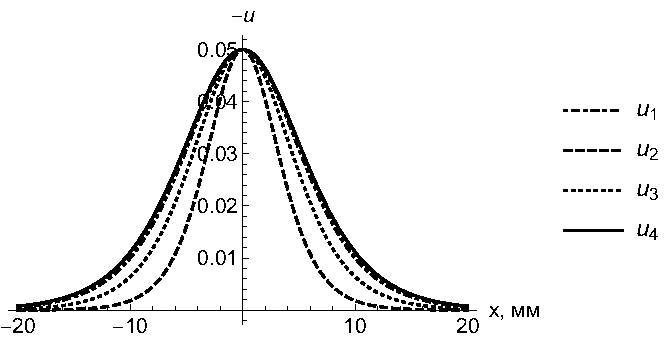
\includegraphics[width=0.54\linewidth]{3a_FourSolitonsBlack}
	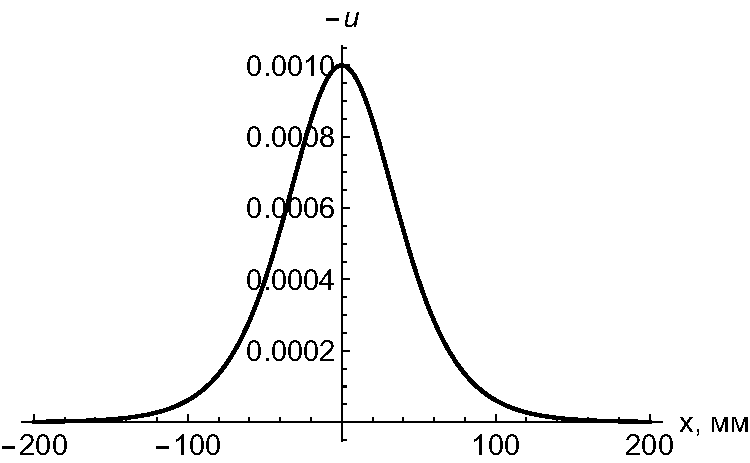
\includegraphics[width=0.42\linewidth]{3b_SingleSoliton}
	\caption{Графики функций $-u_i(x,t)$, задаваемых формулой \eqref{soliton}, в стержне радиуса $R = 5$~мм, сделанном из полистирола при $A = -0.05$ (слева) и $A= -0.001$ (справа).}
	\label{fig:soliton}
	\vspace{-3mm}
\end{figure}
\begin{table}[h]
	\captionsetup{justification=raggedleft,singlelinecheck=false}
	\caption{Упругие модули полистирола.}
	\vspace{-7mm}
	\begin{center}
		\begin{tabular}{|c|c|c|c|c|c|}
			\hline
			\rule[-1ex]{0pt}{3ex} Модуль Юнга & Коэффициент & \multicolumn{3}{|c|} {Модули Мурнагана, Н/м\textsuperscript{2} } & Плотность \\
			\cline{3-5}
			\rule[-1ex]{0pt}{3ex} $E$, Н/м\textsuperscript{2} & Пуассона, $\nu$ & $l$ & $m$ & $n$ & $\rho$, кг/м\textsuperscript{3}  \\
			\hline
			\rule[-1ex]{0pt}{3ex} $3.7\cdot10^9$ & $0.34$ & $-18.9\cdot10^{9}$ & $-13.3\cdot10^{9}$ & $-10\cdot10^{9}$ & 1060 \\
			\hline
		\end{tabular}
	\end{center}
	\label{tab:ps}
	\vspace{-7mm}
\end{table}



\section{Численное моделирование}
Основной интерес для нас представляют непрерывные гладкие решения рассмотренных в предыдущих разделах уравнений, поэтому для численного моделирования мы воспользовались многодоменным псевдоспектральным методом \cite{Canuto2007}, с помощью которого мы решали как полные трёхмерные уравнения \eqref{murnaghan} -- \eqref{full_eqns}, так и одномерное регуляризованное уравнение Буссинеска \eqref{2_eq_fin_reg}. Пример трёхмерной пространственной дискретизации (расположение узлов сетки в стержне) показан на рисунке \ref{fig:grid}.
\begin{figure}[h!]
	\centering
	%\begin{subfigure}{0.5\textwidth}
	\centering
	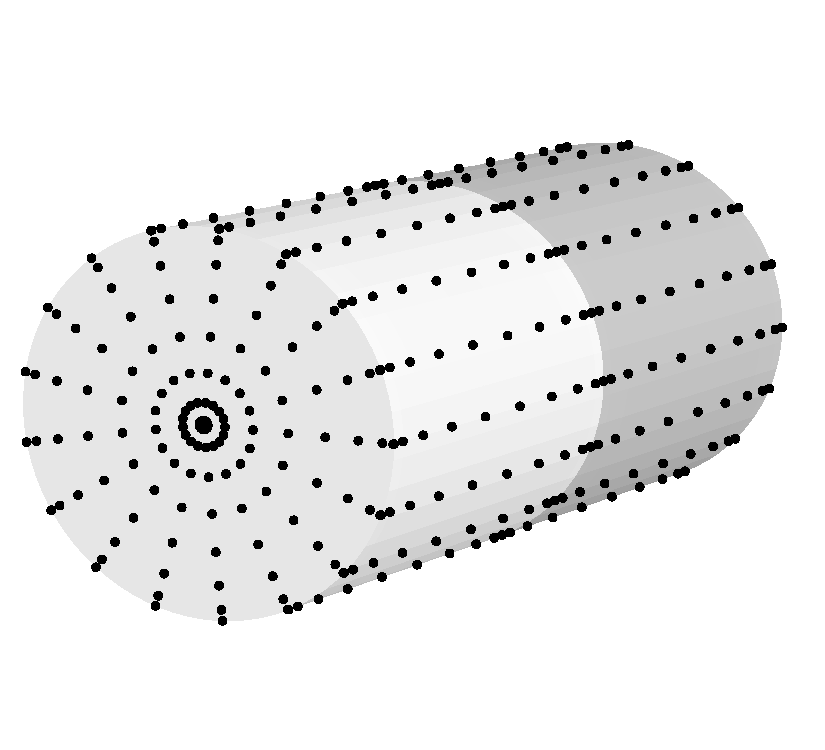
\includegraphics[width=.35\textwidth]{figures/Grid3D}
	%\caption{Lorem ipsum}
	%\end{subfigure}
	%\begin{subfigure}{0.48\textwidth}
	%		\centering
	%		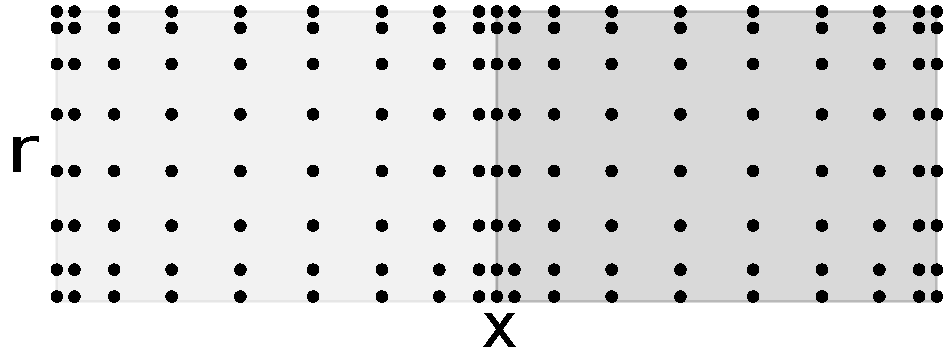
\includegraphics[width=\textwidth]{figures/Grid2D}
	%\caption{Lorem ipsum}
	%	\end{subfigure}
	\caption{Пример трёхмерной сетки из двух доменов, обозначенных разными цветами.}
	\label{fig:grid}
\end{figure}

%Псевдоспектральный метод или метод коллокации, основан на поиске решения задачи в некотором подпространстве, имеющем конечный базис, в качестве которого чаще всего выбирается базис Фурье (набор синусов и косинусов) или семейство ортогональных многочленов. Этот метод используется только для пространственной дискретизации, в то время как дискретизация по времени проводится стандартными методами, например, Рунге-Кутты 4-го порядка. Мы будем использовать псевдоспектральный метод для решения начально-краевых задач как в полной трёхмерной модели \eqref{murnaghan} -- \eqref{full_eqns}, так и в модели Буссинеска. При пространственной дискретизации уравнений Буссинеска (\ref{eq_dim}, $i=1,2$) возникшая система ОДУ оказалась жёсткой и не поддающейся решению явными методами, поэтому в настоящей работе мы проводили моделирование лишь регуляризованного уравнения \eqref{2_eq_fin_reg}.


%\subsection{Образование солитона из длинной волны}
На рисунке \ref{fig:evol_compare} представлено сравнение эволюции заданной в начальный момент времени волны согласно полным уравнениям и регуляризованному уравнению Буссинеска при отсутствии граничных напряжений. В рамках обеих моделей возникают солитоны, двигающиеся быстрее линейной скорости $c=\sqrt{E/\rho}$. В первом случае (левый график) модель Буссинеска дала солитон на 8\% большей амплитуды и, как следствие, бегущий несколько быстрее солитона в полной модели. Во втором случае (правый график), отличающегося от первого большей амплитудой начальной волны, отличие полной модели от модели Буссинеска намного значительнее. 
\begin{figure}[h]
	\centering
	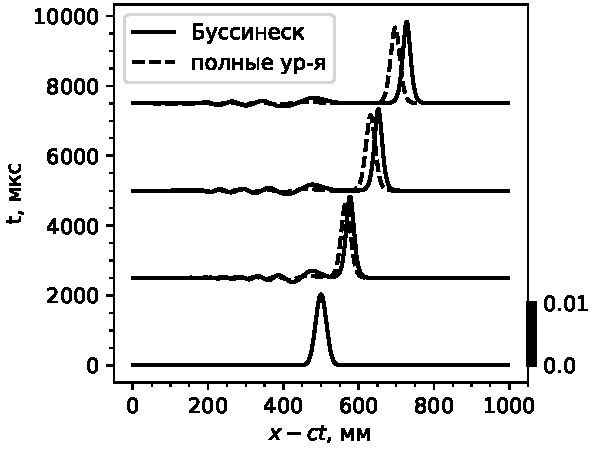
\includegraphics[width=0.44\linewidth]{figures/SolEvolCompareSmall}
	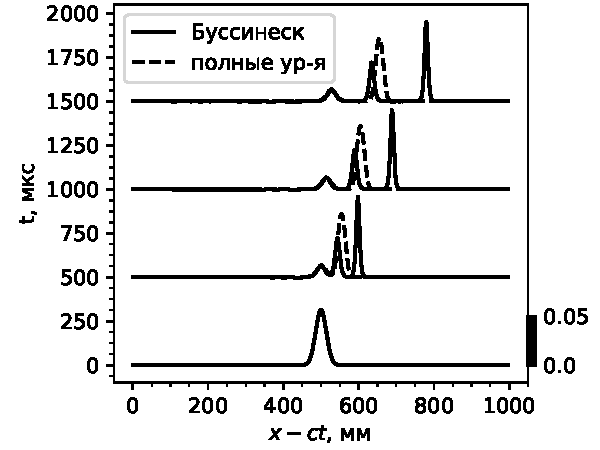
\includegraphics[width=0.44\linewidth]{figures/SolEvolCompareSmall2}
	\caption{Профили решений $-u(x-ct, t)$ регуляризованного уравнения Буссинеска и продольной деформации $-U_x(x - ct, 0, t)$ в центре стержня ($r=0$) в различные моменты времени. Масштаб амплитуды деформации показан чёрным прямоугольником.}
	\label{fig:evol_compare}
	\vspace{-2mm}
\end{figure}

На рисунке \ref{fig:sol_compare} представлено сравнение зависимости скорости солитона от амплитуды в модели Буссинеска \eqref{soliton} и в полной модели. На этом рисунке отчётливо виден асимптотический характер модели Буссинеска.
\begin{figure}[h!]
	\centering
	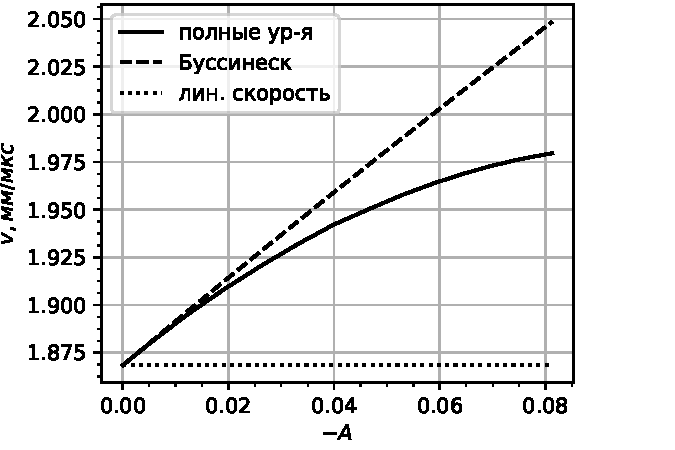
\includegraphics[width=0.53\linewidth]{figures/VelAmplSmall}
	\vspace{-2mm}
	\caption{Зависимость скорости солитона от амплитуды. Горизонтальная линия --- скорость линейных волн $c$.}
	\label{fig:sol_compare}
	\vspace{-3mm}
\end{figure}


%\subsection{Образование солитона из бегущего по поверхности напряжения}
%Выведенная модель типа Буссинеска отличается от полученных ранее учётом напряжения на поверхности. 
%\begin{figure}[h]
%	\centering
%	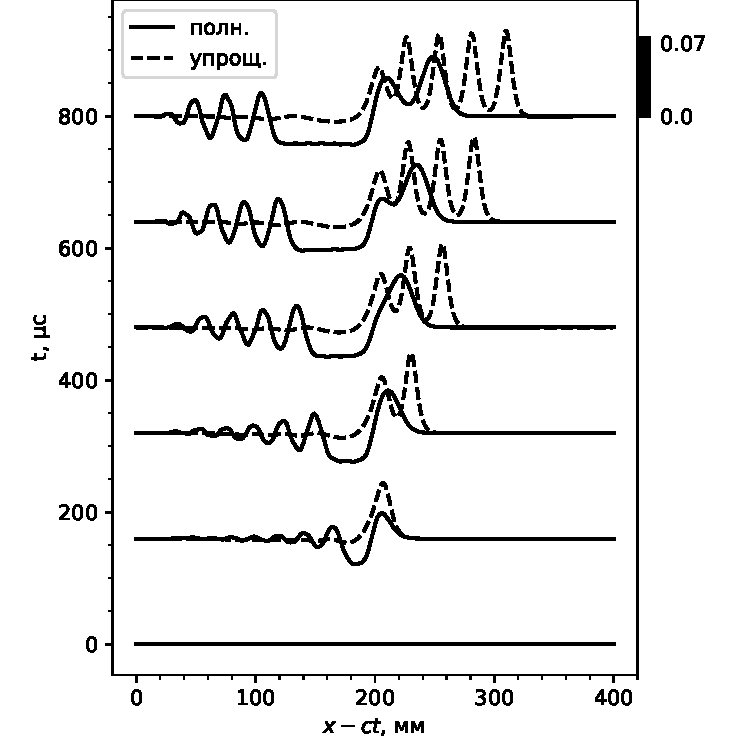
\includegraphics[width=0.49\linewidth]{figures/SolGenForceCompare}
%	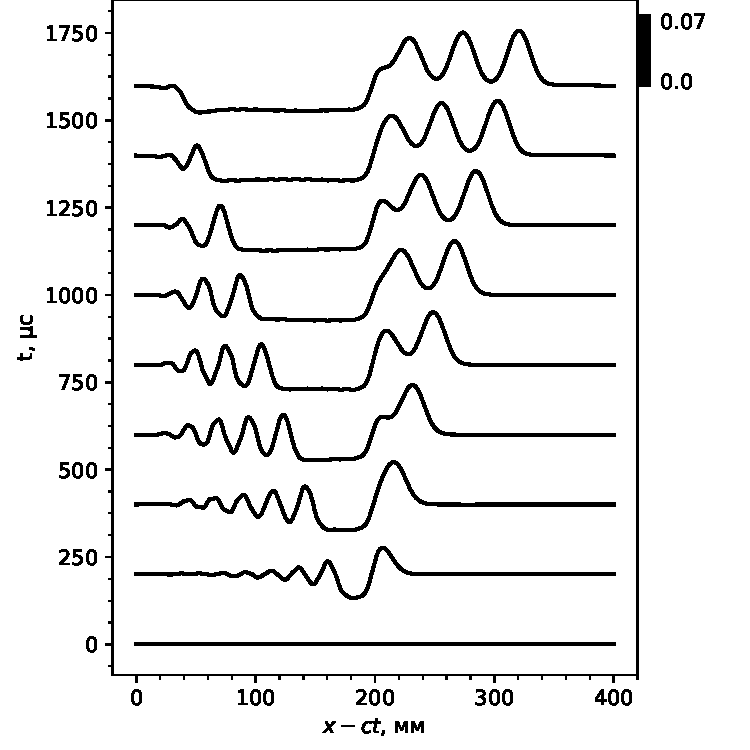
\includegraphics[width=0.49\linewidth]{figures/SolGenForce}
%	\caption{}
%	\label{fig:gen_compar1}
%\end{figure}


Представляет большой интерес возможность возбуждения солитонов в результате внешнего воздействия. На рисунке \ref{fig:impact} представлены результаты моделирования при наличии коротких воздействий (ударов) на торец и на боковую поверхность стержня. Отметим, что в модели Буссинеска стержень предполагается бесконечным и, следовательно, не имеет торцов, однако, мы можем сымитировать удар, задав короткую начальную волну, похожую на ту, что возникает при ударе в полной модели.
\begin{figure}[h!]
	\centering
	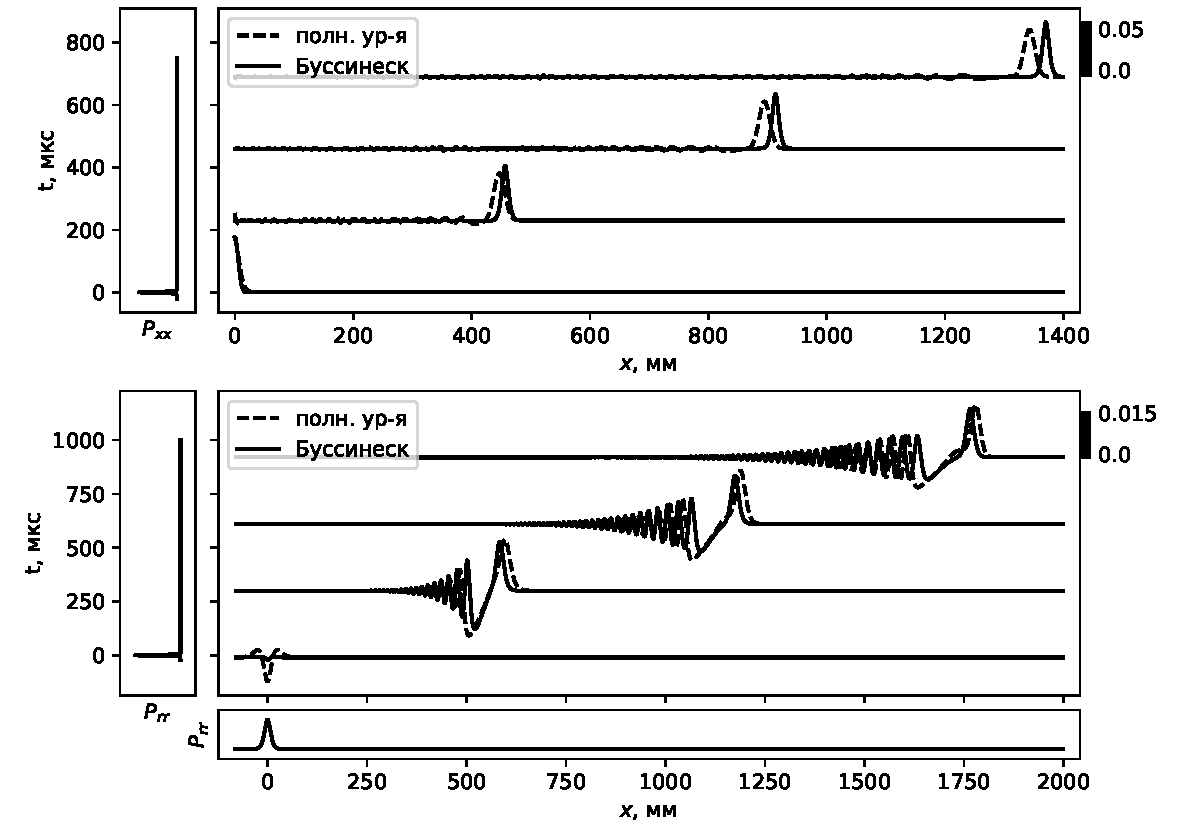
\includegraphics[width=0.85\linewidth]{figures/Impact2Small}
	\caption{Удар по торцу (верхний график) и по боковой поверхности (нижний график) в стержне из полистирола. Вертикальный и горизонтальные подграфики показывают зависимость нормального напряжения на поверхности от времени и координаты $x$. При ударе по торцу напряжение задано одинаковым на всей площади торца.}
	\label{fig:impact}
	\vspace{-1mm}
\end{figure}

На рисунках видно, что модель Буссинеска даёт результаты, схожие с полной моделью. Учитывая, что на рисунках \ref{fig:impact} амплитуды деформации являются достаточно большими в сравнении с пределом упругости и в реальных экспериментах амплитуды как правило на порядок меньше, то можно сделать вывод о хорошей применимости модели Буссинеска для моделирования возникновения солитонов.


%\subsection{О применении полученных результатов для возбуждения солитонов}


%\chapter{Обработка экспериментальных данных}


\section{Заключение}

Для описания продольных длинных волн в стержнях круглого сечения мы вывели две новые асимптотические модели типа Буссинеска, отличающиеся друг от друга коэффициентами при дисперсионных слагаемых. Эти модели обобщены на случай ненулевой осесимметричной нагрузки на боковой поверхности, а также на случай предварительно растянутого стержня.

Нам удалось построить метод, позволяющий численно моделировать полные трёхмерные уравнения движения стержня в рамках нелинейной теории упругости. Мы численно решили ряд начально-краевых задач и показали хорошую применимость модели типа Буссинеска для моделирования возникновения солитонов.

Результаты настоящей работы частично опубликованы в \cite{Garbuzov}.


\let\OLDthebibliography\thebibliography
\renewcommand\thebibliography[1]{
	\OLDthebibliography{#1}
	\setlength{\parskip}{0pt}
	\setlength{\itemsep}{0pt plus 0.3ex}
}

\begin{thebibliography}{99}

	\bibitem{OS} Ostrovsky~L.\,A., Sutin~A.\,M., Nonlinear elastic waves in rods, \textit{PMM} 41 (1977) 531--537.
	\bibitem{NS} Nariboli G.\,A., Sedov A., Burgers-Korteweg de Vries equation for viscoelastic rods and plates, \textit{J. Math. Anal. Appl.} 32~(3) (1970) 661--677.
	\bibitem{S_book} Samsonov A.\,M., Strain solitons in solids and how to construct them, Boca Raton: Chapman \& Hall/CRC, 2001.
	\bibitem{P_book} Porubov A.\,V., Amplification of nonlinear strain waves in solids, Singapore: World Scientific, 2003.	
	%\bibitem{S1} Samsonov~A.\,M., Structural optimization in nonlinear wave propagation problems. In: \textit{Structural Optimization under Dynamical Loading. Seminar and Workshop for Junior Scientists}, U. Lepik ed., Tartu University Press, 75-76 (1982).
	%\bibitem{S2} Samsonov~A.\,M., Soliton evolution in a rod with variable cross section, \textit{Sov. Physics - Doklady} 29 (1984) 586-587.
	\bibitem{SP} Samsonov~A.\,M., Porubov~A.\,V., Refinement of the model for the propagation of longitudinal strain waves in a rod with nonlinear elasticity, \textit{Tech. Phys. Lett.} 19\,(6) (1993) 365--366.
	%\bibitem{PV} Porubov~A.\,V., M.G. Velarde, Dispersive - dissipative solitons in nonllinear solids, \textit{Wave Motion} 31(3) (2000) 197-207.
	\bibitem{DF} Dai~H.-H., Fan~X., Asymptotically approximate model equations for weakly nonlinear long waves in compressible elastic rods and their comparisons with other simplified model equations, \textit{Maths. Mechs. Solids} 9 (2004) 61--79.
	\bibitem{DC} Dai~H.-H., and Z. Cai, Uniform asymptotic analysis for transient waves in a pre-stressed compressible hyperelastic rod, \textit{Acta Mechanica} 139 (2000) 201--230.
	\bibitem{KSZ} Khusnutdinova~K.\,R., Samsonov~A.\,M., A.S. Zakharov, Nonlinear layered lattice model and generalized solitary waves in imperfectly bonded structures, \textit{Phys. Rev. E} 79(5) (2009) 056606.
	\bibitem{KS} Khusnutdinova~K.\,R., Samsonov~A.\,M., Fission of a longitudinal strain solitary wave in a delaminated bar, \textit{Phys. Rev. E} 77 (2008) 066603.
	\bibitem{KT1} Khusnutdinova~K.\,R., Tranter~M.\,R., Modelling of nonlinear wave scattering in a delaminated elastic bar, \textit{Proc. R. Soc. A} 471 (2015) 20150584.
	\bibitem{KT2} Khusnutdinova~K.\,R., Tranter~M.\,R., On radiating solitary waves in bi-layers with delamination and coupled Ostrovsky equations, \textit{Chaos} 27 (2017) 013112.
	\bibitem{JAP2010} Dreiden~G.\,V., Khusnutdinova~K.\,R., Samsonov~A.\,M., and Semenova~I.\,V., Splitting induced generation of soliton trains in layered waveguides, \textit{J. Appl. Phys.} 107 (2010) 034909.
	\bibitem{JAP2012} Dreiden G.\,V., Khusnutdinova~K.\,R., Samsonov~A.\,M., and Semenova~I.\,V., Bulk strain solitary waves in bonded layered polymeric bars with delamination, \textit{J. Appl. Phys.} 112 (2012) 063516.
	\bibitem{Garbuzov} Garbuzov F.\,E., Khusnutdinova K.\,R., Semenova I.\,V., On Boussinesq-type models for long longitudinal waves in elastic rods, \textit{Wave Motion} 88 (2019) 129--143.
	\bibitem{bostrm2000} Bostr\"{o}m A., On wave equations for elastic rods, \textit{ZAMM} 80\,(4) (2000) 245--251. 
	%\bibitem{HughesKelly} Hughes D.\,S., Kelly J.\,L., Second order elastic deformation of solids, Phys. Rev., 1953, 92,  1145-1149.
	\bibitem{Canuto2007} Canuto C. et al., Spectral Methods. Evolution to Complex Geomenties and Applications to Fluid Dynamics, Berlin: Springer-Verlag, 2007.
\end{thebibliography}


%\chapter*{Приложение 1}
%\addcontentsline{toc}{chapter}{Приложение 1}
%%\label{s:appendix_formulas}
%Нелинейные функции в уравнении \eqref{eq2_1}:
%\begin{equation} \nonumber
%\begin{split}
%&\begin{split}
%\Phi_1 =& \, 2\left[(-4\lambda - 4\mu + n - 4m) V_1 - 2(\lambda + 2\mu + m) U_{0x}\right] U_2 \\
%&- \left[ 2(2l + \lambda) V_1 + (3\lambda + 6\mu + 2l + 4m) U_{0x} \right] U_{0xx} \\
%& - \left[ (2\lambda + 2\mu + 8l + n) V_1 + 2(\lambda + \mu + 2l + m) U_{0x} \right] V_{1x},
%\end{split} \\
%&\begin{split}
%\Phi_2 =& \, \frac12 \left[2 (2\lambda + 2\mu + 8l + n) U_{2x} + (4\lambda + 4\mu + 4m - n) V_{1xx} + 32(2\lambda + 3\mu + 2l + 2m) V_3 \right] V_1 \\
%& + 2(\lambda + \mu + 2l + m) U_{0x} U_{2x} + 2(\mu + m)\left[ U_{0xx} + 4 V_{1x} \right] U_2 + (\lambda + 2\mu + m)(U_{0x} V_{1x})_x\\
%& + \frac14(12\lambda + 20\mu + 12m - n) V_{1x}^2 + 8(\lambda + 2l) V_3 U_{0x} + (4\lambda + 12\mu + 4m + n) U_2^2.
%\end{split}
%\end{split}
%\end{equation}
%Функции из формул \eqref{U2}, \eqref{V3}:
%\begin{align}
%\nonumber
%\begin{split}
%f_2(x, t) =& \, \frac{1}{8 \mu ^2} \bigg(U_{0xx} V_1 \left(8\mu^2 - 2\mu(-4\lambda + 4l - 4m + n) + \lambda(4\lambda + 4m - n)\right) \\
%&+ 2V_1 V_{1x} (2 (\lambda + \mu) (2\lambda + \mu) - 8l\mu + 4m(\lambda + \mu) - n(\lambda + 2\mu)) \\
%&+ \rho c^2 U_{0tt}V_1 (-4(\lambda + \mu) - 4m + n) + 2U_{0x}U_{0xx} \left(-2\mu^2 + \mu(\lambda - 2(l + m)) + \lambda (\lambda + m)\right) \\
%&+ 4 U_{0x} V_{1x} \left((\lambda + \mu)^2 - 2l\mu + \lambda m\right) - 2\rho c^2 U_{0x}U_{0tt} (\lambda + 2\mu + m)\bigg)
%\end{split}\\
%\nonumber
%\begin{split}
%f_3(x, t) =& -\frac{1}{8 (\lambda +2 \mu )}\bigg(-\frac{2 V_1 (2 (\lambda +l+m)+3 \mu ) \left(-\rho  s^2 V_{1tt}+2 (\lambda +\mu ) U_{2,x}+\mu  V_{1xx}\right)}{\lambda +2 \mu }\\
%&-\frac{(\lambda +2 l) U_{0x} \left(-\rho  s^2 V_{1tt}+2 (\lambda +\mu ) U_{2x}+\mu  V_{1xx}\right)}{\lambda +2 \mu }+8 l V_1 U_{2x} + (4l + 2m)U_{0x} U_{2x}\\
%&+2 U_2 (\mu +m) \left(U_{0xx}+4 V_{1,x}\right)+m (U_{0x}V_{1x})_x + \lb 3\lambda + 5\mu + 3m -\frac{n}{4}\rb V_{1x}^2\\
%&+\lb 2\lambda + 2\mu + 2m-\frac{n}{2}\rb V_1 V_{1xx}+(2\lambda + 2\mu + n) V_1 U_{2x} + \lambda(U_{0x}V_{1x})_x\\
%&+ 2\mu(U_{0x} V_{1x})_x + (2\lambda + 2\mu)U_{0x}U_{2x} + (4 (\lambda +3 \mu )+4 m+n) U_2^2 \bigg)
%\end{split}
%\end{align}
%Функции из асимптотического представления $V_1$~\eqref{v1_asympt}:
%\begin{align}
%\nonumber
%\begin{split}
%f(x,t) &= \frac{1}{16 (\lambda +\mu )^3 (\lambda +2 \mu )}\bigg(\mu  \rho  s^2 (3 \lambda +2 \mu ) (2 \lambda +3 \mu ) S_{tt}+\lambda  \mu  (\lambda +2 \mu ) (3 \lambda +2 \mu ) S_{xx}\\
%&\hspace{25mm}+(\lambda +\mu ) \left(\mu  (\lambda +2 \mu ) (4 \lambda +3 \mu ) U_{0xxx}-\rho c^2 \left(3 \lambda ^2+7 \lambda  \mu +3 \mu ^2\right) U_{0xtt}\right)
%\end{split}\\
%\nonumber
%\begin{split}
%g(x,t) &= -\frac{1}{8(\lambda + \mu)}\bigg(-\frac{2U_{0x}(\lambda + 4l - 2m + n) \left(\lambda(\lambda + \mu) U_{0x} - \mu S (3\lambda + 2\mu)\right)}{(\lambda + \mu)^2} + \\
%&\hspace{20mm}\frac{(3 (\lambda +\mu )+4 l+2 m) \left(\mu  S (3 \lambda +2 \mu )-\lambda  (\lambda +\mu ) U_{0,x}\right){}^2}{(\lambda +\mu )^4} + (4l + 2\lambda)  U_{0x}^2\bigg)
%\end{split}
%\end{align}
%
%\chapter*{Приложение 2.\\Солитонные решения уравнения типа Буссинеска}
%\addcontentsline{toc}{chapter}{Приложение 2}
%%All Boussinesq-type equations discussed in the paper can be cast in the form
%Все уравнения типа Буссинеска, обсуждавшиеся в настоящей работе, могут быть записаны в виде:
%\begin{equation}
%u_{tt} - c^2 u_{xx} = \tilde{\beta} (u^2)_{xx} + \tilde\alpha_1 u_{tttt} + \tilde\alpha_2 u_{ttxx} + \tilde\alpha_3 u_{xxxx},
%\end{equation}
%где $c$, $\tilde\beta$ и $\tilde\alpha_i$ -- некоторые постоянные. Будем искать решения в виде волн, бегущих влево или вправо:$ u = u(\xi), \; \mbox{где} \; \xi = x \pm vt, $
%что сводит исходное уравнение к обыкновенному дифференциальному уравнению:
%\begin{equation}
%(v^2 - c^2) u'' = \tilde\beta (u^2)'' + (\tilde\alpha_1 v^4 + \tilde\alpha_2 v^2 + \tilde\alpha_3) u^{IV}.
%\label{ODE}
%\end{equation}
%Интегрируя это уравнения по $\xi$ дважды и требуя, чтобы на бесконечности не было возмущений $u, u', u'', u''' \to 0$ при $\xi \to \pm \infty$, получаем уравнение:
%\begin{equation}
%u'' = \frac{(v^2-c^2) u - \tilde\beta u^2}{\tilde\alpha_1 v^4 + \tilde\alpha_2 v^2 + \tilde\alpha_3},
%\end{equation}
%которое может рассматриваться как уравнение движения частицы единичной массы в поле потенциальной силы. Интеграл энергии имеет вид:
%%which can be viewed as Newton's equation of motion for a particle of unit mass in a potential field. The energy integral has the form
%\begin{equation}
%E = \frac 12 \left (u' \right )^2 - \frac{3 (v^2-c^2) u^2 - 2 \tilde\beta u^3}{6 (\tilde\alpha_1 v^4 + \tilde\alpha_2 v^2 + \tilde\alpha_3)},
%\end{equation}
%а солитонное решение соответствует нулевому уровню энергии $E=0$. Разделение переменных позволяет получить солитонное решение в виде:
%\begin{equation} \label{4_soliton}
%u = \frac{3 (v^2 - c^2)}{2 \tilde\beta} \sech^2 \left [\sqrt{\frac{v^2 - c^2}{4 (\tilde\alpha_1 v^4 + \tilde\alpha_2 v^2 + \tilde\alpha_3)}} (x \pm v t)\right ]
%\end{equation}
%для таких значений параметра $v$, что это решение вещественнозначное.
%Решение \eqref{4_soliton} можно репараметризовать через амплитуду $A$:
%\begin{equation}
%u = A \sech^2 \left [\sqrt{\frac{3A\tilde{\beta}}{2 (\tilde\alpha_1 (3c^2+2A\beta)^2 + 3\tilde\alpha_2 (3c^2+2A\beta) + 9\tilde\alpha_3)}} \lb x \pm t\sqrt{c^2+\frac23A\beta} \rb\right ].
%\end{equation}
	
\end{document}